\documentclass[conference,a4paper]{IEEEtran}
\IEEEoverridecommandlockouts
\usepackage[utf8]{inputenc}
\usepackage[T1]{fontenc}
\usepackage{cite}
\usepackage{amsmath,amssymb}
\usepackage{graphicx}
\usepackage{booktabs}
\usepackage{tabularx}
\usepackage{xcolor}
\usepackage{tikz}
\usetikzlibrary{positioning,arrows.meta}
\usepackage{url}
\usepackage[hidelinks]{hyperref}
\renewcommand{\arraystretch}{1.12}
\newcolumntype{Y}{>{\raggedright\arraybackslash}X}

\begin{document}

\title{ITAS-MM: An Intelligent Multimodal Traffic Assistance System for Real-Time Traffic Sign Recognition, Lane Detection, and Legally Grounded Driving Guidance}

\author{\IEEEauthorblockN{Tran Anh Kiet (SE182050), Phan Khanh Bang (SE180630), Cao Tran Tien (SE184692)}
\IEEEauthorblockA{FPT University, Vietnam}}

\maketitle

\begin{abstract}
Driver assistance systems that recognize traffic signs usually stop at a class label and leave the driver to work out what the sign requires. This paper presents ITAS-MM, a research prototype that recognizes Vietnamese traffic signs in forward-camera video or still images, links each confirmed sign to passages of the governing regulations, and reads the result aloud in Vietnamese. The system separates localization from classification: a single-class YOLO11n detector finds sign panels, and a MobileNetV3-small classifier assigns one of 87 codes of the national standard QCVN 41:2024 or rejects the crop. On video, codes are confirmed only after consistent evidence over several frames, using a label-independent track association and a per-track voting rule. The models were trained on 15,603 images merged from five public data sets with lineage-grouped splits. Fine-tuning raised detector recall on the test split from 0.851 to 0.875 and mAP50 from 0.919 to 0.936, with paired bootstrap intervals that exclude zero, and the recognizer reaches 0.970 accuracy on crops of 32 pixels and above. On fifteen one-minute field segments, the temporal module reduced fragmented tracks by 38\% and, together with a lower video threshold, raised the number of coded tracks from 75 to 96. The results also show the limits of the prototype: detector precision falls from 0.923 on curated data to 0.641 on real driving video, and small or nighttime signs remain the main source of error.
\end{abstract}

\begin{IEEEkeywords}
traffic sign recognition, object detection, temporal voting, legal information retrieval, Vietnamese text-to-speech
\end{IEEEkeywords}

\section{Introduction}

Road traffic crashes kill about 1.19 million people every year \cite{who2023}. A large part of this risk comes from drivers who miss or misread information that is already present on the road, such as a prohibition sign partly hidden by a truck or a warning sign seen too late at night. Camera-based driver assistance can help, and traffic sign recognition is one of its most studied components. However, most recognition pipelines end with a class name. A label such as P.106a is of little use to a driver who does not remember that it prohibits trucks, and it says nothing about the legal rule behind the sign.

Vietnam is a demanding setting for this problem. Its sign catalog, defined in the national technical regulation QCVN 41:2024 \cite{qcvn41}, contains many visually similar codes, and urban roads are dense with motorcycles, advertising boards and signs mounted at varied heights. Recent work on Vietnamese roads reports that small and distant signs are the main weakness of single-pass detectors \cite{nguyen2025}. At the same time, research on Vietnamese legal question answering has shown that traffic regulations can be retrieved and cited automatically \cite{lexisign,graphsign,vlsp2025}, but these systems work from typed questions rather than from what a camera sees.

This paper describes ITAS-MM, a prototype that connects these two lines of work. Given an uploaded video or image, it detects sign panels, assigns QCVN codes, confirms them across frames, retrieves the relevant passages from official legal documents and produces a short spoken observation in Vietnamese. The system is deliberately cautious. It does not claim that a sign legally applies to the driver, and it reports uncertain cases as unrecognized rather than guessing.

The paper makes three contributions. First, it describes a two-stage sign pipeline in which a class-agnostic detector is followed by an 87-code classifier with an explicit background class, so that localization does not depend on the size of the code vocabulary and uncertain crops can be rejected. Second, it introduces a simple temporal evidence module that associates detections across frames without relying on their labels and confirms a code only when it clearly leads the other candidates. Third, it reports an evaluation that pairs standard data set metrics with measurements on real driving video, which exposes a domain gap that data set metrics alone would hide.

The rest of the paper is organized as follows. Section~\ref{sec:related} reviews related work. Section~\ref{sec:data} describes the data. Section~\ref{sec:method} presents the models and the temporal module, and Section~\ref{sec:impl} describes how they are packaged into a web application. Section~\ref{sec:exp} reports the experiments, Section~\ref{sec:discussion} discusses the findings and limitations, and Section~\ref{sec:conclusion} concludes.

\section{Related Work}\label{sec:related}

\textit{Traffic sign detection.} Traffic sign detection has moved from hand-crafted color and shape features to end-to-end deep learning, and YOLO-family detectors are now the usual choice for real-time use. Their accuracy drops sharply for small objects, which is critical for signs seen from a distance. Slicing-aided hyper inference (SAHI) addresses this by running the detector on overlapping tiles of a high-resolution image and merging the results \cite{sahi}. Nguyen et al. \cite{nguyen2025} confirm the small-sign problem on Vietnamese urban data. Unlike approaches that train one detector for all codes, ITAS-MM detects panels with a single-class model and leaves the code to a separate classifier, which allows codes to be added without retraining the detector.

\textit{Lane detection.} Lane detection shifted from pixel-wise segmentation to row-wise classification, which is faster and handles occlusion better. Ultra Fast Lane Detection and its successor formulate lanes as selections over predefined row anchors \cite{ufld,ufldv2}. ITAS-MM uses UFLD-v2 for a visual lane overlay only, because no Vietnamese lane ground truth was available to validate lane geometry for legal use.

\textit{Legal question answering.} The VLSP 2025 shared task on multimodal legal question answering over traffic sign regulation \cite{vlsp2025} has produced training-free multi-stage pipelines \cite{lexisign} and graph-based retrieval systems \cite{graphsign}. These systems answer questions about images and regulations, but they are evaluated as standalone question-answering tasks. ITAS-MM uses a lighter lexical retriever and drives it from the codes confirmed by the vision pipeline.

\textit{Spoken and multimodal assistance.} Vietnamese neural text-to-speech is available as open software \cite{vieneu}, and multimodal assistants that combine vision and speech have been built for visually impaired users \cite{naviblind} and for driver warnings based on large language models \cite{xu2024}. Studies of driver response show that auditory and multimodal warnings can reduce cognitive load compared with visual alerts alone \cite{politis}. ITAS-MM follows this direction with short, neutral spoken observations rather than commands.

\section{Data}\label{sec:data}

\subsection{Sources and merging}

The sign data set merges five public Vietnamese traffic sign collections, four published on Kaggle and one on Roboflow Universe, listed in Table~\ref{tab:sources}. Together they provide 29,599 images and 60,580 annotated boxes, but they overlap heavily: one Kaggle collection is itself an earlier export of the Roboflow project, and many images are consecutive frames of driving videos. Each image therefore keeps its provenance, exact duplicates are merged into one canonical image whose boxes keep the list of source annotations they came from, and the resulting localization set contains 15,603 images and 30,558 boxes, about half of the raw total.

Splits were made by group rather than by image. Images that share content or lineage, such as frames of the same video, receive a common split group, and a whole group is assigned to one split, so that near-duplicate frames never appear in more than one split. This gives 10,952 training, 2,325 validation and 2,326 test images. The split fingerprints are frozen, and the test split was never used for model selection or threshold tuning.

\begin{table}[t]
\centering
\caption{Source collections and their share of the merged set}
\label{tab:sources}
\begin{tabular}{lrrr}
\toprule
Source & Raw images & Raw boxes & Merged images \\
\midrule
Kaggle, lapnguyen2003 & 10,157 & 19,748 & 8,158 \\
Kaggle, thaivothanh & 10,933 & 20,583 & 1,633 \\
Kaggle, namvipcf2000 & 3,659 & 11,514 & 2,030 \\
Roboflow, v6 export & 3,680 & 5,894 & 2,914 \\
Kaggle, jaydenguyenx & 1,170 & 2,841 & 868 \\
\midrule
Total & 29,599 & 60,580 & 15,603 \\
\bottomrule
\end{tabular}
\end{table}

\subsection{Recognition labels}

The recognition labels were built in two steps. An initial manifest covers 30 codes with 10,003 crops. The ontology was then extended to 87 QCVN codes. Boxes outside the original 30 codes were labeled by two independent passes of an AI-assisted labeling procedure that compared each crop with the official figure of the regulation. A box was kept only when both passes agreed, which retained 976 boxes (raw agreement 76.9\%) and excluded 555. The final recognizer was trained on 17,445 training and 3,933 validation crops whose native short side is at least 16 pixels, while the test split keeps all sizes. Because these labels were not reviewed by independent human annotators, accuracies measured on them describe agreement with the labeling procedure rather than expert accuracy.

\subsection{Exploratory analysis}

Table~\ref{tab:sizes} shows the distribution of box sizes, measured by the shorter side of each box. The data are dominated by small signs: about 27\% of training boxes and 31\% of test boxes are shorter than 16 pixels, and only about one box in five is 64 pixels or larger. Because recognition becomes unreliable below about 16 pixels, as shown in Section~\ref{sec:exp}, a large share of the boxes can be localized but not read. Class support is also uneven. In the 71-class labeling of the original release, the speed limit sign P.127 alone has 2,123 training boxes, followed by the no-stopping and no-parking signs P.130 and P.131a with 1,325 and 1,219, while several classes have fewer than ten training boxes. In the final 87-code recognizer, 55 codes have enough training data to be treated as main classes and 32 low-support classes are trained but reported separately.

\begin{table}[t]
\centering
\caption{Number of boxes by shorter side (pixels)}
\label{tab:sizes}
\begin{tabular}{lrrrrr}
\toprule
Split & $<16$ & 16 to 32 & 32 to 64 & $\geq 64$ & Total \\
\midrule
Train & 5,635 & 5,986 & 5,251 & 4,051 & 20,923 \\
Validation & 1,336 & 1,535 & 1,089 & 787 & 4,747 \\
Test & 1,502 & 1,306 & 1,180 & 900 & 4,888 \\
\bottomrule
\end{tabular}
\end{table}

\subsection{Field video and legal corpus}

Two further sources were used for evaluation on real video. A field pilot of 120 frames with 66 signs from one development driving video provides human-reviewed boxes, although sign codes were not reviewed. Three field evaluation videos recorded in Hanoi, two by day and one at night, were cut into fifteen segments of 60 seconds. These segments carry no annotation and are used to measure behavior such as track counts and speed. Finally, the legal corpus consists of Law No.~36/2024/QH15 \cite{law36}, Decree No.~168/2024/ND-CP \cite{decree168} and QCVN 41:2024 \cite{qcvn41}, indexed as 703 page-grounded passages from four official PDF files.



\section{Methodology}\label{sec:method}

\subsection{System overview}

Fig.~\ref{fig:arch} shows the pipeline. An uploaded video is decoded frame by frame and analyzed at 6 Hz. For each analyzed frame, the detector proposes sign panels, the recognizer assigns a code to each panel, and the temporal module decides which codes are confirmed. Confirmed codes are used to retrieve legal passages and to produce spoken cues, and the system writes a result video with the overlays and a timed list of signs. A still image follows the same path without the temporal step. The lane model runs in parallel and provides visual context only.

\begin{figure*}[t]
\centering
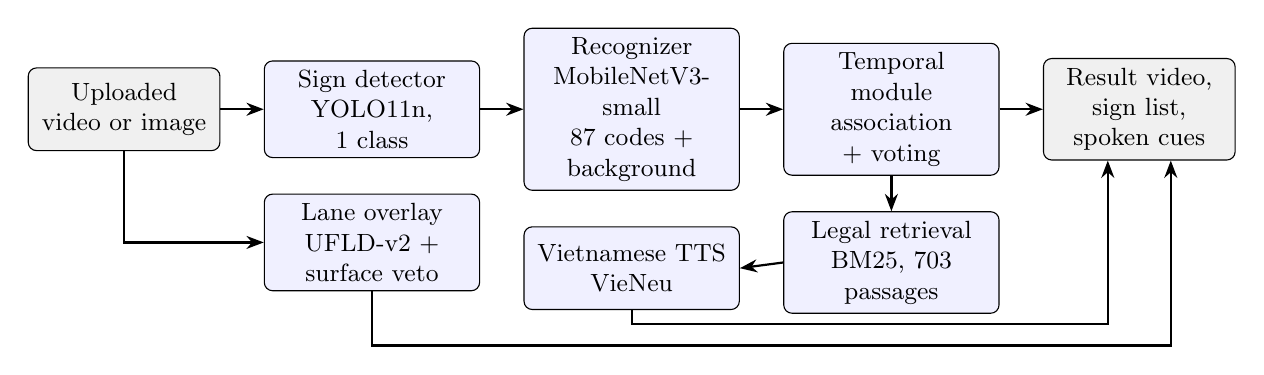
\begin{tikzpicture}[node distance=0.45cm and 0.55cm,
  box/.style={draw,rounded corners=3pt,align=center,minimum height=1.05cm,text width=2.5cm,font=\small,fill=blue!6},
  io/.style={draw,rounded corners=3pt,align=center,minimum height=1.05cm,text width=2.2cm,font=\small,fill=gray!12},
  arr/.style={-{Stealth[length=2.2mm]},thick}]
\node[io] (in) {Uploaded video or image};
\node[box,right=of in] (det) {Sign detector\\YOLO11n, 1 class};
\node[box,right=of det] (rec) {Recognizer\\MobileNetV3-small\\87 codes + background};
\node[box,right=of rec] (tmp) {Temporal module\\association + voting};
\node[io,right=of tmp] (out) {Result video, sign list, spoken cues};
\node[box,below=of det] (lane) {Lane overlay\\UFLD-v2 + surface veto};
\node[box,below=of tmp] (law) {Legal retrieval\\BM25, 703 passages};
\node[box,below=of rec] (tts) {Vietnamese TTS\\VieNeu};
\draw[arr] (in) -- (det);
\draw[arr] (det) -- (rec);
\draw[arr] (rec) -- (tmp);
\draw[arr] (tmp) -- (out);
\draw[arr] (in.south) |- (lane.west);
\draw[arr] (tmp.south) -- (law.north);
\draw[arr] (law.west) -- (tts.east);
\draw[arr] (lane.south) |- ([yshift=-4.5mm]tts.south) -| ([xshift=4mm]out.south);
\draw[arr] (tts.south) -- ([yshift=-1.8mm]tts.south) -| ([xshift=-4mm]out.south);
\end{tikzpicture}
\caption{Overview of ITAS-MM. Signs are analyzed at 6 Hz on video; the lane overlay is used for display only and does not influence sign decisions.}
\label{fig:arch}
\end{figure*}

\subsection{Detection and recognition}

The detector is YOLO11n with 2.59 million parameters, trained with a single-class so that it learns what a sign panel looks like regardless of its code. It runs at 640 pixels on images and at 960 pixels with an additional 640 pixel view on video, which helps with small signs. Each detected panel is cropped, resized to 128 pixels and passed to a MobileNetV3-small classifier with 1.56 million parameters. The classifier outputs a probability $p(c \mid x)$ for each of the 87 codes and for a background class $\varnothing$ that absorbs crops that are not signs or not in the vocabulary. A crop is assigned a code only when
\begin{equation}
\hat{c} = \arg\max_{c}\, p(c \mid x) \neq \varnothing \quad \text{and} \quad p(\hat{c} \mid x) \geq \tau ,
\label{eq:accept}
\end{equation}
otherwise it is reported as unrecognized. The threshold $\tau$ is 0.87 for still images, calibrated on the validation split, and 0.64 for video, where the temporal module provides additional evidence. The raw top-1 label and its score are kept for every crop, so a rejection can always be explained.

\subsection{Temporal evidence on video}

A single frame can misread a sign because of blur, occlusion or distance, so video decisions are made per physical sign rather than per frame. The module first associates each detection with an existing track. A detection $s$ joins track $k$ if their boxes overlap with an intersection over union of at least 0.3. When the overlap is too small, which is common for fast-moving signs at 6 Hz, a label-independent fallback accepts the pair if
\begin{equation}
\Delta t \leq T, \qquad \frac{1}{2} \leq \frac{A_s}{A_k} \leq 2, \qquad \lVert \mathbf{c}_s - \mathbf{c}_k \rVert \leq d_k ,
\label{eq:assoc}
\end{equation}
where $\Delta t$ is the time since the track was last seen, $T = 0.75$ s, $A$ denotes box area, $\mathbf{c}$ the box center and $d_k$ the diagonal of the track box. Fallback pairs are assigned one-to-one in order of increasing distance, so that one track never absorbs two neighboring signs. Because the fallback ignores labels, a sign that is still unrecognized keeps its identity while it approaches the camera.

Each track then collects the codes accepted by \eqref{eq:accept} within the last $T$ seconds. Let $n_k(c)$ be the number of such votes for code $c$. The leading code $c^{*}$ is confirmed when
\begin{equation}
n_k(c^{*}) \geq m \quad \text{and} \quad n_k(c^{*}) > \max_{c \neq c^{*}} n_k(c),
\label{eq:vote}
\end{equation}
with $m = 3$ for uploaded video. Unrecognized samples cast no vote, so a single misread no longer cancels a confirmed code, while hard vetoes such as an unsupported symbol shape clear the votes of a track. This design replaces an earlier rule that reset the vote count whenever a new label appeared, which made confirmation fragile for small signs.

\subsection{Legal retrieval and speech}

For each confirmed code, the system queries the legal corpus with the code and its Vietnamese name. Passages are ranked with BM25 \cite{robertson2009} using $k_1 = 1.2$ and $b = 0.75$, complemented by half-weighted bigram and trigram matches that favor passages quoting the exact sign name. Retrieval returns page-grounded quotations with links to the source document and never generates legal text. Spoken output uses the open VieNeu model \cite{vieneu}. Each confirmed sign produces one cue at the moment of confirmation, and cues closer than 1.5 s are merged into one sentence of at most two signs so that stacked signs are not dropped. The wording is a neutral observation, stating only that the system may have seen a given sign, and it never instructs the driver.

\subsection{Training}

The detector was trained in three successive stages on the same YOLO11n model, summarized in Table~\ref{tab:stages}. The first stage started from public pretrained weights and trained for 20 epochs without augmentation to obtain a stable baseline. The second stage applied light color and scale augmentation with a small learning rate. The third stage, which produced the final model, used AdamW with a learning rate of $10^{-3}$ decayed to one hundredth, a batch of 16 images at 640 pixels, mixed precision and mild geometric and color augmentation, and took 23 minutes on a laptop GPU with 4 GB of memory. Horizontal flipping was disabled, because a mirrored left-turn sign is a valid right-turn sign with a different meaning, and mosaic augmentation was off in the final stage. Each stage selected its checkpoint on the validation split only.

\begin{table}[t]
\centering
\caption{Detector training stages}
\label{tab:stages}
\begin{tabularx}{\columnwidth}{llY}
\toprule
Stage & Epochs, optimizer & Augmentation \\
\midrule
1. Baseline & 20, default, lr 0.01 & none \\
2. Retraining & 8, AdamW, lr $10^{-4}$ & light color and scale \\
3. Fine-tuning & 10, AdamW, lr $10^{-3}$ & color, rotation $2^\circ$, translation, scale \\
\bottomrule
\end{tabularx}
\end{table}

The recognizer was trained for 30 epochs with AdamW and a one-cycle schedule at a peak learning rate of $4\times10^{-4}$, a batch of 128 and 14,000 crops sampled per epoch, with sampling weights that favor rare classes. It was initialized from the earlier 30-code model, so that the original classes keep their learned features while the 57 new codes are added. The checkpoint was selected by the main-class macro F1 score on the validation split and the acceptance threshold was calibrated on the same split. Retraining from scratch on the same machine reproduced the validation macro F1 to within 0.0011 and selected the same epoch and threshold.

\section{System Implementation}\label{sec:impl}

The models are packaged as a local web application with a Python backend built on FastAPI and a single-page frontend built with React. Two workflows are offered. For an image, the frontend sends the file to an analysis endpoint and receives the detected panels, their codes and confidences, an annotated image and the spoken text, which is synthesized only when the user asks for it. For a video, the upload is stored and processed as a background job. The server accepts MP4 files of up to 850 MB and 100,000 frames, refuses a second job while one is running, and reports progress that the frontend converts into an estimated remaining time.

The video job reads every source frame in order, runs the full pipeline on the analyzed frames and draws the overlays on the frames that are written to the result video. Between two analyzed frames, the boxes and lane lines are moved with the image content so that the overlay stays aligned. When the job ends, the result video is decoded again from start to finish, and it is published only if the number of decoded frames matches the number written. The job also records, for every confirmed sign, the time at which it was confirmed; the frontend plays the corresponding spoken cue when the result video reaches that time and clears pending cues when the user seeks.

Profiling showed that the lane models and the drawing and encoding of output frames dominated the processing time, while sign detection and recognition took less than a tenth of it. Two changes were therefore made. The result video is written at 30 frames per second instead of the source rate of 60, and the lane overlay is recomputed on every second analyzed frame, that is at 3 Hz, while signs are still analyzed at 6 Hz. On a 90 s night clip these changes reduced the processing time from 406 s to 165 s, and the sign boxes and labels were identical in all 540 analyzed frames before and after the change.

Fig.~\ref{fig:ui} shows the interface after a video has been processed. The result video is shown next to a timed list of confirmed signs; selecting a time moves the video to that moment, and each sign can be expanded to show the cited legal passage with a link to the source document.

\begin{figure}[t]
\centering
\includegraphics[width=\columnwidth]{ui_video_result_desktop.png}
\caption{Web application after processing an uploaded night clip: result video with overlays, voice toggle and timed list of confirmed signs.}
\label{fig:ui}
\end{figure}

\section{Experiments}\label{sec:exp}

\subsection{Setup and metrics}

Detection is evaluated on the test split at a confidence of 0.35, a non-maximum suppression threshold of 0.45 and a matching threshold of 0.5 intersection over union, using precision, recall, mAP50 and mAP50-95 with 101-point interpolation. The difference between two detectors is assessed with a paired bootstrap over test images with 1,000 resamples, and an improvement is accepted when its 95\% interval excludes zero. Recognition is evaluated on crops of ground-truth boxes, grouped by crop size, using accuracy and macro F1. On the field segments, where no ground truth exists, we report the number of tracks, the number of tracks that received a code, the number of distinct codes and the processing speed. Retrieval is evaluated on 24 development queries with Recall@k and mean reciprocal rank. All experiments ran on a laptop with an NVIDIA RTX 3050 GPU with 4 GB of memory.

\subsection{Detection}

Table~\ref{tab:det} compares the baseline and the fine-tuned detector. Fine-tuning improved every metric. The paired bootstrap gives a recall gain of 0.0245 (95\% interval 0.0170 to 0.0317) and an mAP50 gain of 0.0163 (0.0122 to 0.0198), so both improvements are statistically supported. As Fig.~\ref{fig:size}a shows, the gain is concentrated where it matters most: recall for boxes below 16 pixels rose from 0.651 to 0.713, while boxes of 32 pixels and above were already detected with a recall of about 0.96.

Localization quality is good at the usual matching threshold but loose at strict thresholds. As Fig.~\ref{fig:det}a shows, the average precision of the fine-tuned model stays above 0.85 up to an intersection over union of 0.75 and then falls quickly, to 0.660 at 0.85, 0.414 at 0.90 and 0.063 at 0.95. The boxes are therefore accurate enough to crop a sign for recognition but not pixel tight, which explains the gap between mAP50 (0.936) and mAP50-95 (0.736). Fig.~\ref{fig:det}b shows the validation metrics during the final fine-tuning stage. The best mAP50-95 was reached at the last of the ten epochs, so a longer schedule might still improve the model.

\begin{figure*}[t]
\centering
\begin{minipage}{0.48\textwidth}\centering
\includegraphics[width=\linewidth]{fig3_detector_ap_by_iou.png}\\
\small (a) Average precision across IoU thresholds
\end{minipage}\hfill
\begin{minipage}{0.48\textwidth}\centering
\includegraphics[width=\linewidth]{fig4_detector_finetuning_curve.png}\\
\small (b) Validation metrics during the final fine-tuning stage
\end{minipage}
\caption{Detector localization and training behavior. Precision and recall stay high up to IoU 0.75; the final fine-tuning stage was still improving at its last epoch.}
\label{fig:det}
\end{figure*}

\begin{table}[t]
\centering
\caption{Detector results on the test split}
\label{tab:det}
\begin{tabular}{lcccc}
\toprule
Model & Precision & Recall & mAP50 & mAP50-95 \\
\midrule
Baseline & 0.923 & 0.851 & 0.919 & 0.717 \\
Fine-tuned & \textbf{0.936} & \textbf{0.875} & \textbf{0.936} & \textbf{0.736} \\
\bottomrule
\end{tabular}
\end{table}

\begin{figure*}[t]
\centering
\begin{minipage}{0.48\textwidth}\centering
\includegraphics[width=\linewidth]{fig2_detector_recall_by_size.png}\\
\small (a) Detector recall by box size
\end{minipage}\hfill
\begin{minipage}{0.48\textwidth}\centering
\includegraphics[width=\linewidth]{fig5_recognizer_by_crop_size.png}\\
\small (b) Recognizer accuracy and macro F1 by crop size
\end{minipage}
\caption{Performance by object size on the test split. Both models are reliable for signs of 32 pixels and above and degrade for small signs.}
\label{fig:size}
\end{figure*}

\subsection{Recognition}

On test crops of 32 pixels and above, the 87-code recognizer reaches an accuracy of 0.970 and a macro F1 of 0.959, compared with 0.937 and 0.906 for the earlier 30-code model on the same crops. Over all crop sizes its accuracy is 0.909, against 0.790 for the earlier model, and the largest improvement occurs below 16 pixels, where accuracy rose from 0.514 to 0.784 (Fig.~\ref{fig:size}b). Table~\ref{tab:op} shows the effect of the acceptance threshold. Lowering $\tau$ from 0.87 to 0.64 increases coverage from 90.4\% to 96.2\% of crops while the share of correct answers among accepted crops drops only from 98.9\% to 98.3\%, which motivated the lower threshold on video.

\begin{table}[t]
\centering
\caption{Recognizer operating points on test crops of 32 pixels and above (30-code subset)}
\label{tab:op}
\begin{tabular}{lccc}
\toprule
Setting & Coverage & Correct/acc. & Correct/all \\
\midrule
Earlier model, $\tau = 0.63$ & 0.975 & 0.956 & 0.932 \\
87-code model, $\tau = 0.87$ & 0.904 & 0.989 & 0.893 \\
87-code model, $\tau = 0.64$ & 0.962 & 0.983 & 0.945 \\
\bottomrule
\end{tabular}
\end{table}

Performance is uneven across classes. Among the 41 classes with at least 20 test crops, the median accuracy is 0.911 and 23 classes reach 0.90 or more. The weakest classes are W.205a (0.143), R.301c (0.280) and W.203a (0.442), all of which belong to families of visually similar variants. Several of the weakest codes were added by the ontology extension, so part of their error may come from label noise rather than from the model.

The extension also helped the original classes. In the earlier model, errors were concentrated in visually similar pairs: on crops of 32 pixels and above, the no-left-and-right-turn sign P.137 was predicted correctly in only 17 of 73 crops and confused with the no-right-turn sign P.123b in 39 of them. Table~\ref{tab:pairs} shows that the 87-code model, trained with crops down to 16 pixels and with the extended ontology, reduced most of these confusions.

\begin{table}[t]
\centering
\caption{Accuracy of frequently confused classes, all test crop sizes}
\label{tab:pairs}
\begin{tabular}{lccc}
\toprule
Code & Test crops & Earlier model & 87-code model \\
\midrule
P.137 & 87 & 0.345 & 0.897 \\
P.123b & 97 & 0.691 & 0.918 \\
W.201a & 49 & 0.531 & 0.857 \\
W.203c & 16 & 0.875 & 0.875 \\
\bottomrule
\end{tabular}
\end{table}

\subsection{Reliability of the labels}

Because no independent human annotation was available, two independent AI-assisted reviewers labeled a sealed, shuffled set of 885 crops without seeing each other's answers or the model predictions. Agreement was measured with exact label agreement and Cohen's kappa, with ``uncertain'' and ``not a sign'' treated as categories. Agreement was 0.829 (kappa 0.805) on crops from the Hanoi field video, 0.723 (0.693) on the test boxes added by the ontology extension and 0.684 (0.625) on the development video. Agreement depends strongly on size: on the field crops it rises from 0.775 for crops of 16 to 32 pixels to 0.971 for crops of 64 pixels and above, and on the extension test boxes from 0.470 to 0.864. Labels of large signs are therefore reliable, while labels of small signs, and the metrics computed on them, carry substantial uncertainty.

\subsection{Temporal evidence on field video}

Table~\ref{tab:field} reports four configurations on the same fifteen field segments. Comparing the first two rows isolates the effect of the new association and voting rule at the original threshold of 0.87. The number of tracks fell from 1,205 to 846, and tracks with fewer than three samples fell from 1,022 to 637, a reduction of 38\%. Fewer fragments mean that the evidence for one physical sign is no longer split across several short tracks. The number of coded tracks, however, did not change at this threshold. The remaining rows show that the threshold, not the tracker, limited how many signs were coded: lowering $\tau$ to 0.75 and then to 0.64 raised the coded tracks to 86 and 96 and the distinct codes to 20 and 23.

\begin{table}[t]
\centering
\caption{Behavior on fifteen 60 s field segments at 6 Hz}
\label{tab:field}
\begin{tabular}{lcccc}
\toprule
Configuration & Tracks & Coded & Codes & FPS \\
\midrule
Previous tracker, $\tau=0.87$ & 1,205 & 75 & 15 & 2.82 \\
New tracker, $\tau=0.87$ & 846 & 75 & 15 & 3.05 \\
New tracker, $\tau=0.75$ & 839 & 86 & 20 & 3.00 \\
New tracker, $\tau=0.64$ & 834 & 96 & 23 & 3.01 \\
\bottomrule
\end{tabular}
\end{table}

Because the field segments have no ground truth, the 52 tracks that the 0.64 setting adds over 0.87 were graded by inspecting their best crop. Of these, 39 were correct, 4 were wrong and 9 could not be decided from the crop, which gives a precision of 90.7\% on the decided tracks, or 75.0\% if every undecided track is counted as wrong. Fig.~\ref{fig:examples} shows typical cases. The correct tracks include large, clear prohibition and information signs, while the wrong ones include a blue map pin on an advertisement read as a roundabout sign, a taxi prohibition read as a general car prohibition, and a crop that contains two stacked signs.

\begin{figure}[t]
\centering
\includegraphics[width=\columnwidth]{fig_track_examples.png}
\caption{Best crops of tracks added by the lower video threshold. Top: correct codes. Bottom: wrong codes and an undecidable crop.}
\label{fig:examples}
\end{figure} An earlier comparison on a different field population had favored the stricter threshold (precision 0.963 against 0.887), so the choice of 0.64 is a deliberate trade of precision for coverage that should be revisited with more graded data.

Fig.~\ref{fig:three} illustrates the effect on a difficult night scene with three signs stacked on one pole. The previous configuration read none of them. The final configuration reads the pedestrian prohibition P.112 and the slow-down warning W.245a. The third sign receives top-1 scores between 0.13 and 0.51 and remains unread under either threshold, which points to the recognizer rather than the decision rule.

\begin{figure}[t]
\centering
\includegraphics[width=\columnwidth]{fig_three_signs_baseline_vs_final.png}
\caption{Night scene with three stacked signs. Red boxes: previous configuration, no code read. Green boxes: final configuration, which reads P.112 and W.245a.}
\label{fig:three}
\end{figure}

\subsection{Domain gap}

Table~\ref{tab:pilot} reports the detector on the 120-frame field pilot. Fine-tuning reduced false positives from 28 to 19 while keeping recall, which raised precision from 0.641 to 0.729. The improvement is consistent with the test split, but the absolute numbers are far lower: the same baseline detector has a precision of 0.923 on the curated test data and 0.641 on real driving video. The pilot is small, with 66 signs from a single video, so these figures indicate the size of the gap rather than measure it precisely.

\begin{table}[t]
\centering
\caption{Detector on the field pilot (120 frames, 66 signs)}
\label{tab:pilot}
\begin{tabular}{lccccc}
\toprule
Model & TP & FP & FN & Precision & Recall \\
\midrule
Baseline & 50 & 28 & 16 & 0.641 & 0.758 \\
Fine-tuned & 51 & 19 & 15 & 0.729 & 0.773 \\
\bottomrule
\end{tabular}
\end{table}

\subsection{Legal retrieval}

On the 24 development queries, the retriever reaches a Recall@1 of 0.542, a Recall@3 of 0.833, a Recall@4 of 0.875 and a mean reciprocal rank of 0.684. The correct passage is therefore usually among the first three results but often not the first one.

Table~\ref{tab:legal} shows the top-ranked passages for four signs, queried as the web application does, with the code followed by its Vietnamese name. In all four cases the first result is a passage from the appendix of QCVN 41:2024 that describes neighboring codes, because the appendix repeats sign codes and names densely and BM25 rewards these repetitions. The articles that define the meaning of prohibition and warning signs appear at ranks two or three. For the user this means that the relevant rule is usually visible after expanding the result, but the first passage can be misleading. Boosting passages that contain the exact queried code, or indexing each sign definition as its own passage, are simple remedies that were not evaluated in this work.

\begin{table}[t]
\centering
\caption{Top-ranked passages for four sign queries}
\label{tab:legal}
\begin{tabularx}{\columnwidth}{lYY}
\toprule
Query & Rank 1 & General sign article \\
\midrule
P.106a, no trucks & appendix passage on turn bans & Art.~22, rank 2 \\
P.112, no pedestrians & appendix passage on P.111 & Art.~22, rank 3 \\
W.245a, go slowly & appendix passage on W.211 & Art.~28, rank 2 \\
P.131a, no parking & appendix passage on zone plates & Art.~22, rank 2 \\
\bottomrule
\end{tabularx}
\end{table}

\subsection{Runtime}

On the development GPU the fine-tuned detector needs 10.8 ms per image, the recognizer 0.12 ms per crop in batches of 50, and the complete per-image pipeline, including lane detection and retrieval, 46.2 ms. Uploaded video is slower than this per-image figure suggests, because every source frame must be decoded and every output frame drawn and encoded. With the settings of Section~\ref{sec:impl}, a 90 s clip is processed in 165 s, or 1.8 times its duration.

\section{Discussion}\label{sec:discussion}

The experiments support three observations. First, separating detection from classification worked well on curated data. The detector reaches high recall for medium and large signs, the classifier is accurate above 32 pixels, and the background class gives a natural way to reject crops that do not belong to the vocabulary. Second, the temporal module is most useful as a way to keep evidence together. It cut fragmented tracks by more than a third, but it could not create codes that the recognizer did not propose, so coverage on video is ultimately bounded by recognition quality on small, blurred and dark crops. Third, data set metrics overstate field performance. The drop from 0.923 to 0.641 precision between curated test images and real driving video is the most important result for anyone who would deploy such a system.

\textit{Threats to validity.} Several aspects of the evaluation limit how far the results generalize. The test split is drawn from the same five public collections as the training data, so it shares their cameras, regions and labeling conventions even though near duplicates were separated. The field segments come from three videos recorded in one city, and neighboring segments of the same video are correlated, so the 15 segments are not 15 independent samples. The track grading and the label reliability study rely on AI-assisted review, and their agreement with expert annotators has not been measured. Finally, the video threshold was chosen after observing the field segments on which it is evaluated, which can make the reported coverage gain optimistic.

The work has several limitations that follow from these observations. The recognizer covers 87 codes, which is only part of the QCVN 41:2024 catalog, and 32 of them have little training data. The labels for the extended codes and the precision figures on field video come from AI-assisted review rather than independent human annotation, and the field samples are small.

The lane overlay has no Vietnamese ground truth, does not distinguish dashed from solid markings and is never used to decide which sign applies to the vehicle. Supplementary panels that restrict a sign by time, vehicle type or distance are not interpreted in the final version: an optical character recognition component read a distance panel correctly in a test, but its parser covered only time windows and vehicle types and night panels were unreadable, so it was disabled and sign applicability is reported as uncertain. Uploaded video is processed about 1.8 times slower than real time, a real-time streaming mode was prototyped but not retained, and the position input is simulated rather than taken from GPS. Finally, retrieval sometimes ranks a general article above the article that defines the detected sign, and the legal corpus has not been checked for current legal effect. In addition, the models were not compared with other published methods on a common public benchmark, because the merged data set, its 87-code ontology and the field video differ from those used in prior work; the reported gains are therefore relative to the project's own baselines. For these reasons ITAS-MM must be understood as a research prototype and not as a driving-safety system or a source of legal advice.

\section{Conclusion}\label{sec:conclusion}

This paper presented ITAS-MM, a prototype that turns forward-camera video into confirmed Vietnamese traffic sign codes, cited legal passages and short spoken observations. A single-class detector, an 87-code classifier with a background class and a label-independent temporal module together achieve strong results on curated data and a measurable improvement in the stability of video decisions. The evaluation also shows clearly where the approach falls short: small and nighttime signs, a sizable gap between curated and real video, and the absence of human ground truth for field accuracy.

Future work should first build a source-disjoint field test set with human-reviewed boxes, codes and lanes, so that field precision and recall can be measured rather than estimated. Recognition of small signs could be improved with tiled inference and additional training crops between 16 and 32 pixels, and the most confused pairs need targeted data. Beyond recognition, the system would benefit from more output classes, a stronger multi-object tracker, lane markings classified as dashed or solid, supplementary-panel reading with its own test set, real GPS input and an optimized runtime that allows real-time streaming on embedded hardware. The source code, configuration and evaluation scripts are available at \url{https://github.com/BANGPC123/itas-mm-scaffold}.

\begin{thebibliography}{99}
\bibitem{who2023} World Health Organization, \emph{Global Status Report on Road Safety 2023}. Geneva, Switzerland: WHO, 2023.
\bibitem{qcvn41} Ministry of Transport of Vietnam, \emph{QCVN 41:2024/BGTVT, National Technical Regulation on Road Signs and Markings}, 2024.
\bibitem{nguyen2025} D. Nguyen, H. V. Dung, V.-T.-L. Le, and T. Doan, ``Traffic sign detection in Vietnam: An experimental study,'' in \emph{Proc. 18th National Conf. on Fundamental and Applied Information Technology Research}, 2025.
\bibitem{lexisign} P. X. Pham, D. Q. Le, T. H. Tran, and T. N.-T. Huynh, ``LexiSignVQA: A unified training-free multi-stage approach to multimodal legal question answering on traffic sign rules,'' in \emph{Proc. VLSP}, 2025.
\bibitem{graphsign} H. M. Huynh, A. N. T. Khuong, D. P. Trong, and T. V. Huynh, ``Reading the signs: A graph-based system for multimodal information retrieval on Vietnamese traffic law,'' in \emph{Proc. VLSP}, 2025.
\bibitem{vlsp2025} S. T. Luu \emph{et al.}, ``VLSP 2025 MLQA-TSR challenge: Vietnamese multimodal legal question answering on traffic sign regulation,'' 2025.
\bibitem{sahi} F. C. Akyon, S. O. Altinuc, and A. Temizel, ``Slicing aided hyper inference and fine-tuning for small object detection,'' in \emph{Proc. IEEE Int. Conf. Image Processing (ICIP)}, 2022, pp. 966-970.
\bibitem{ufld} Z. Qin, H. Wang, and X. Li, ``Ultra fast structure-aware deep lane detection,'' in \emph{Proc. European Conf. Computer Vision (ECCV)}, 2020.
\bibitem{ufldv2} Z. Qin, P. Zhang, and X. Li, ``Ultra fast deep lane detection with hybrid anchor driven ordinal classification,'' \emph{IEEE Trans. Pattern Anal. Mach. Intell.}, 2022.
\bibitem{vieneu} pnnbao97, ``VieNeu-TTS: A Vietnamese neural text-to-speech system,'' GitHub repository, 2024.
\bibitem{naviblind} M.-Q. Tran, D. Truong, D.-T. Pham, and M.-A. Nguyen, ``NaviBlind: A multimodal AI assistant for visually impaired users to identify product information from images and speech,'' 2025.
\bibitem{xu2024} Z. Xu, T. Chen, and S. Chen, ``A LLM-based multimodal warning system for driver assistance,'' 2024.
\bibitem{politis} I. Politis, S. Brewster, and F. Pollick, ``Age, cognitive load, and multimodal effects on driver response to directional warning,'' 2017.
\bibitem{law36} National Assembly of Vietnam, \emph{Law on Road Traffic Order and Safety}, Law No. 36/2024/QH15, 2024.
\bibitem{decree168} Government of Vietnam, \emph{Decree No. 168/2024/ND-CP on Administrative Penalties for Road Traffic Order and Safety Violations}, 2024.
\bibitem{robertson2009} S. Robertson and H. Zaragoza, ``The probabilistic relevance framework: BM25 and beyond,'' \emph{Foundations and Trends in Information Retrieval}, vol. 3, no. 4, pp. 333-389, 2009.
\end{thebibliography}

\end{document}
